\begin{figure}[!h]
\centering
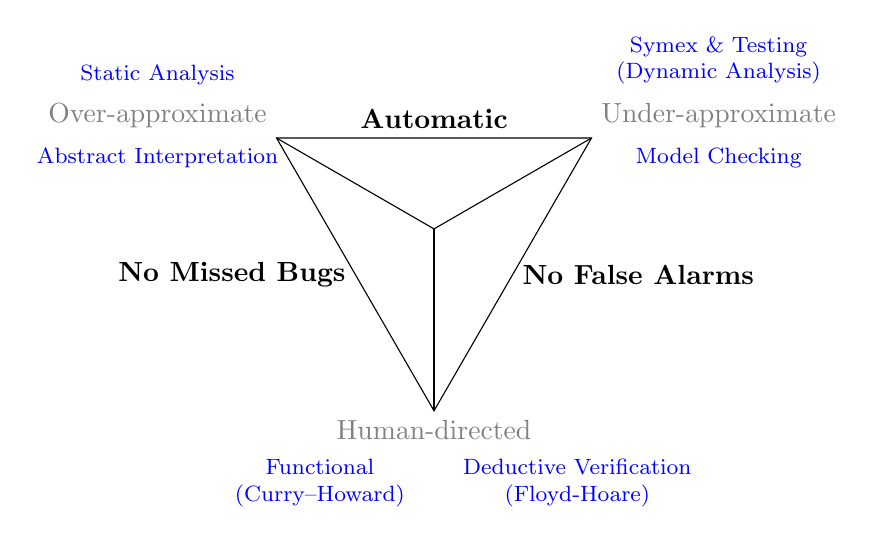
\begin{tikzpicture}
\draw (0,{sqrt(12)}) node[anchor=south east, label=above:{\color{blue} \footnotesize Static Analysis}, label=below:{\color{blue} \footnotesize Abstract Interpretation}] {\color{gray} Over-approximate}
  -- (2,0) node[anchor=north, label={[align=center, text=blue, font=\footnotesize]below left:Functional\\(Curry–Howard)}, label={[align=center, text=blue, font=\footnotesize]below right:Deductive Verification\\(Floyd-Hoare)}] {\color{gray} Human-directed} node[midway, left]{\textbf{No Missed Bugs}}
  -- (4,{sqrt(12)}) node[anchor=south west, label={[align=center, text=blue, font=\footnotesize]above:Symex \& Testing\\(Dynamic Analysis)}, label=below:{\color{blue} \footnotesize Model Checking}] (UA) {\color{gray} Under-approximate} node[midway, right]{\textbf{No False Alarms}}
  -- cycle node[midway, above]{\textbf{Automatic}};

\draw [-] (0, {sqrt(12)}) to (2, 2.31);
\draw [-] (2, 0) to (2, 2.31);
\draw [-] (4, {sqrt(12)}) to (2, 2.31);


% \pgfmathparse{sqrt(12)}
% \node (A) {A};
% \node [right=4cm of A] (B) {B};
% \node [below right=\pgfmathresult cm and 2cm of A] (C) {C};


% \draw [-] (A) to (B) node[midway, right]{this works};
% \draw [-] (B) to (C) node[midway, right]{this works};
% \draw [-] (A) to (C) node[midway, right]{this works};
  
%   \node[fill=blue,circle,text width=3cm] (first) at (1,1) {First};
% \node[fill=green,circle,text width=3cm] (second) at (5,5) {This is the text that will be cover with the connection lines};
% \node[fill=purple,circle,text width=3cm] (third) at (1,9) {This text will be covered too};
% % insert connection lines in background using myback layer

% \draw (first.east) to (third.east);
% \draw (first.west) to (third.north east);

\end{tikzpicture}
\caption{The Triangle Model of Software Verification adapted from the paper by M. Brain and D. Kroening \cite{TSVP}.}
\label{fig:tmsv}
\end{figure}